
\chapter{Wings of War}

\section{The board game}

Wings of War is a game series which merges card and board game mechanics to recreate aerial combat.

Airplanes are represented by a single card which is used as a playing piece on any open surface; the players choose and \textbf{play simultaneously} movement cards to decide the actions of the airplane they control. Different planes use different decks of movement cards to represent their different maneuver capabilities, and different decks of ``Fire'' card are used to take into account their fighting effectiveness and to keep track of damages.

Each Wings of War set is a complete game for 2 to 4 players which may be combined with additional sets, or with other copies of the same set, to play larger games.

\begin{figure}
  \centering
      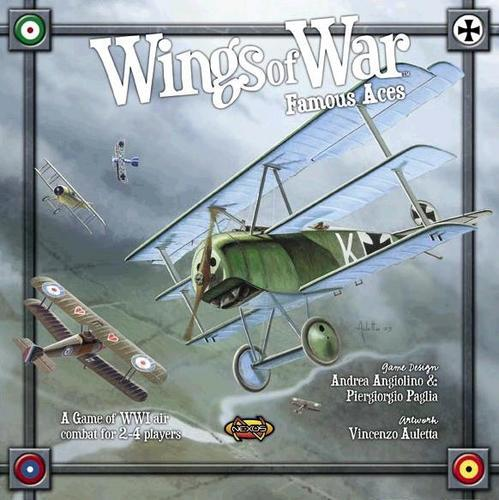
\includegraphics[width=0.5\textwidth]{images/wow.jpg}
  \caption{Wings Of War box}
\end{figure}

\section{Basic Rules}
\subsection{Preparation}
Each player chooses an equal number of airplane cards then he takes a gameboard for each plane and puts on it, in the proper place, a set of “Maneuver” cards, matching the blue letter on the airplane card.
The game can be played with more than one plane per player: maneuver planning, firing and damage account are made separately for each airplane. It is also possible to play with more than two players, divided into teams.
\subsection{Game turn}
Each turn has a planning phase and three movement \& fire phases.
\subsection{Planning}
 At the start of the turn, each player chooses three cards from each of his planes’ maneuver decks. These cards are the three maneuvers that each plane will perform during that turn.
Certain maneuver cards need to be played after (or before) some specific cards.
\subsection{Movement}
When all the players have planned their moves, they reveal the first of their Maneuver cards for the turn (then the second and the third, in the same order of choice).
The planes are then moved using the right rigid cardboard guides.
\subsection{Firing}
After all planes have moved using their maneuver cards the players have to check if an airplane can fire at an opponent’s airplane using the rigid ruler. If the check is positive the airplane can fire at the opponent. It is possible that two planes can fire at each other. 
If the target airplane is reached by the first half of the ruler, it takes two cards of damage. If it is more distant and it is reached by the second half of the ruler, it takes only one card of damage. Fighter airplanes can fire at a single target each phase. It is forbidden to fire through another plane, enemy or friendly.
\subsection{Damage}
When an airplane is fired at, the owner of that plane takes the damage cards and secretly looks at them and adds them to the previous damages the plane suffered. When the total reaches or excedes the life points on the airplane card, the airplane is shot down and eliminated.
Only if the player draws a card with the cross symbol must he reveal it and the airplane that fired at him has jammed his guns and cannot fire after each of the next three maneuvers.
\textbf{All damage is resolved simultaneously} after all airplanes that can fire have fired. Therefore, a plane that is shot down may still fire the same phase in which it is shot down.
\subsection{Rest of the turn}
Each turn is composed of three game phases. After all airplanes that can fire have resolved their firing, the first game phase is ended. Everybody reveals the second maneuver card for the  turn. Move and resolve firing. Then reveal the third card, move  and resolve firing. Then the turn is finished and the planning  of the next one can begin.
\subsection{Overlapping}
If two airplane cards overlap, neither of the two airplanes can fire at each other until they move and don’t overlap any more. They can, however, still fire at other planes. Other planes can shoot at the overlapping planes using the normal rules.
\subsection{Exit from the gaming surface}
An airplane that goes out of the playing area with its central dot is out of the game.
\subsection{Victory}
The last player having one or more planes on the playing area after all the enemy ones have been eliminated or exited wins the match.

\section{Our game}
\label{modify this name} 
Our customization to game rules were made to simplify the game flow.

In a nutshell:
\begin{itemize}
    \item Two players (Ai vs Human), one plane each.
    \item Reduced set of maneuver cards
    \item Only two cards per turn have to be chosen
    \item Every shot always hits the target
    \item Damage is fixed, no short/long range differentiation
    \item No overlapping related rules
    \item Exiting from the \textit{world} is a sudden death (and a game over)           
\end{itemize}

\subsection{Cards}
In the planning phase each player has to choose \textbf{two} from the available cards.

Available cards are:
\begin{itemize}
    \item Long/short forward thrust
    \item Long/short right turn
    \item Long/short left turn
\end{itemize}
